\documentclass[problem]{mcs}

\begin{pcomments}
  \pcomment{CP_build_MSTs}
  \pcomment{ARM 10/27/11}
  \pcomment{F11.cp9m, F15.cp8w}
  \pcomment{figure addded, revised ARM 10/21/15}
\end{pcomments}

\pkeywords{
 spanning_tree
 weighted_tree
 minimum_weight
 MST
}

%%%%%%%%%%%%%%%%%%%%%%%%%%%%%%%%%%%%%%%%%%%%%%%%%%%%%%%%%%%%%%%%%%%%%
% Problem starts here
%%%%%%%%%%%%%%%%%%%%%%%%%%%%%%%%%%%%%%%%%%%%%%%%%%%%%%%%%%%%%%%%%%%%%

\begin{problem}
Let $G$ be the $4 \times 4$ grid with vertical and horizontal edges
between neighboring vertices and edge weights as shown in
Figure~\ref{fig:4x4}.

In this problem you will practice some of the ways to build minimum
weight spanning trees.  For each part, list the edge weights in the
order in which the edges with those weights were chosen by the given
rules.

\iffalse
  Formally,
\[
\vertices{G} = [0,3]^2 \eqdef \set{(k,j) \suchthat 0 \leq k,j \leq 3}.
\]
Letting $h_{i,j}$ be the horizontal edge $\edge{(i,j)}{(i+1,j)}$ and
$v_{j,i}$ be the vertical edge $\edge{(j,i)}{(j,i+1)}$ for $i\in[0,2],
j \in [0,3]$, the weights of these edges are
\begin{align*}
w(h_{i,j}) & \eqdef  \frac{4i+j}{100},\\
w(v_{j,i}) & \eqdef 1+\frac{i+4j}{100}.
\end{align*}
\fi

%\begin{center}
\begin{figure}[h]
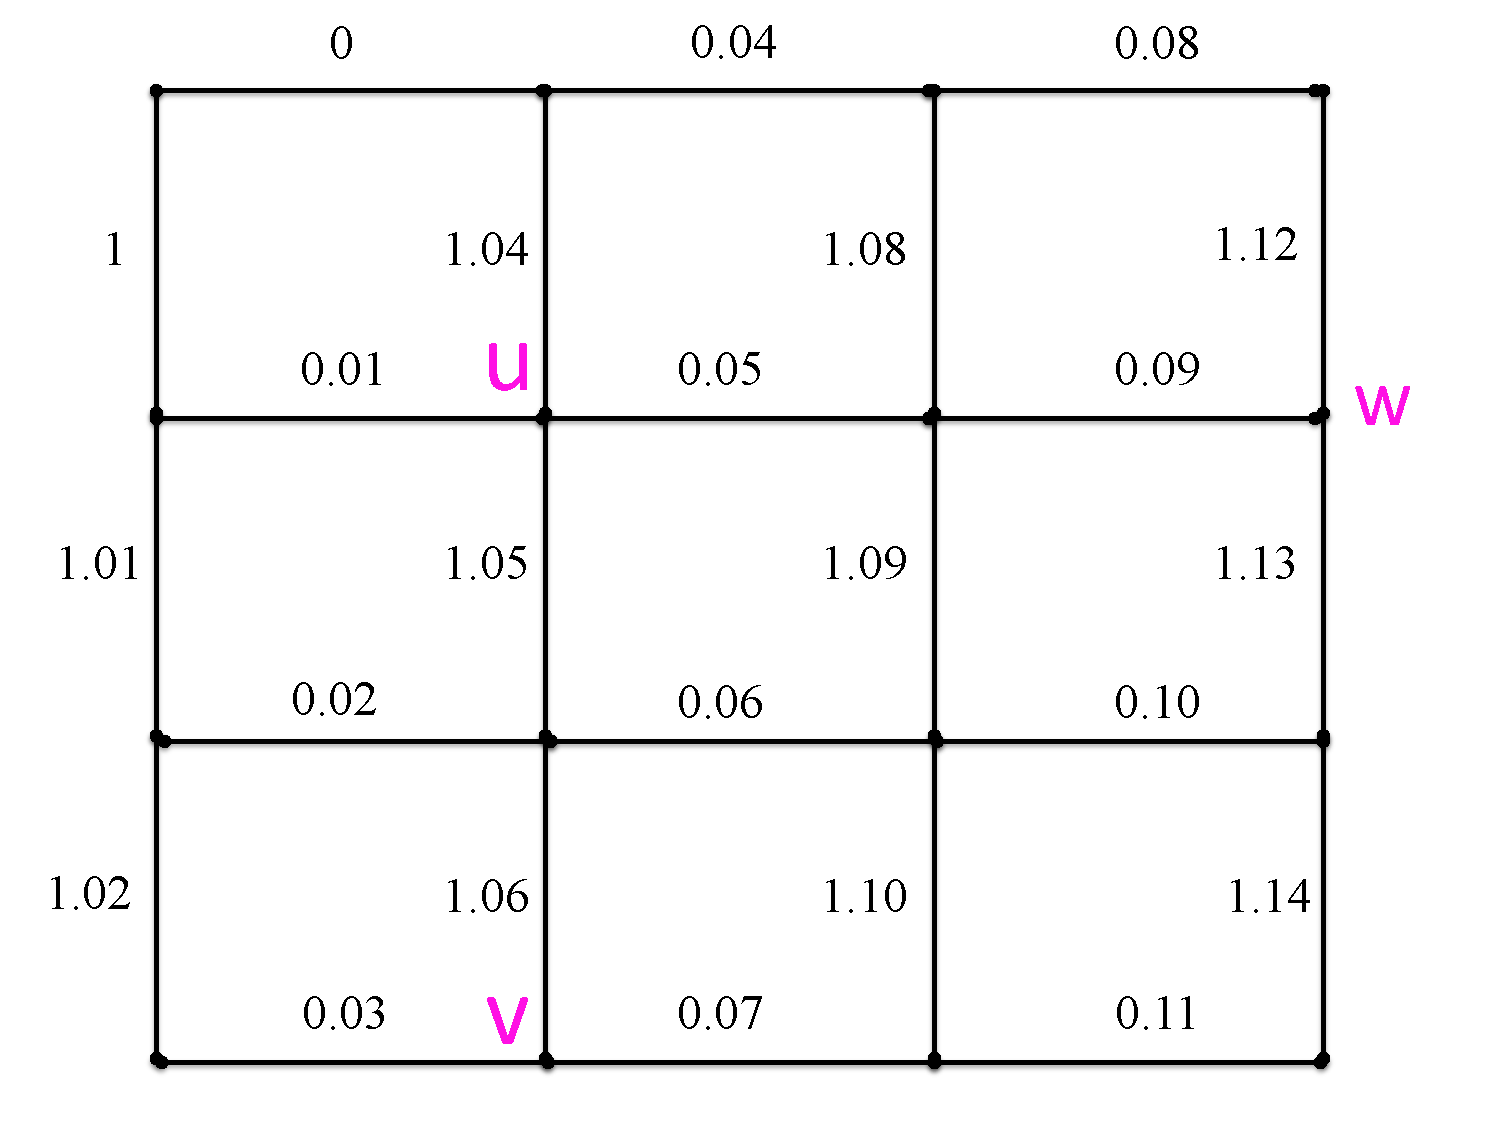
\includegraphics[height=4in]{4x4-array.pdf}
\caption{The 4x4 array graph $G$}
\label{fig:4x4}
\end{figure}
%\end{center}

\bparts

\ppart Construct a minimum weight spanning tree (MST) for $G$ by
initially selecting the minimum weight edge, and then successively
selecting the minimum weight edge that does not create a cycle with
the previously selected edges.  Stop when the selected edges form a
spanning tree of $G$.  (This is Kruskal's MST algorithm.)

\inhandout{For any step in Kruskal's procedure, describe a black-white
  coloring of the graph components so that the edge Kruskal chooses is
  the minimum weight ``gray edge'' according to
  Lemma~\bref{lem:edgeextends}.}

\begin{staffnotes}
Students are often unclear about the ``gray edge'' rule.  If the
problem drags, coaches can explain how the rule applies here and in
the next part, and let students work it out for the last part.
\end{staffnotes}

\begin{solution}

\begin{staffnotes}
\inhandout{From the text: An edge does not create a cycle iff it
  connects different components.  The edge chosen by Kruskal's
  algorithm will become the minimum weight gray edge of a black-white
  coloring when the components it connects are assigned different
  colors.}
\end{staffnotes}

\[
0,\ .01,\ .02,\ .03,\ .04,\ .05,\ .06,\ .07,\ .08,\ .09,\ .10,\ .11,\ 1,\ 1.01,\ 1.02
\]

\end{solution}

\ppart Grow an MST for $G$ by starting with the tree consisting of the
single vertex $u$ and then successively adding the minimum weight edge
with exactly one endpoint in the tree.  Stop when the tree spans $G$.
(This is Prim's MST algorithm.)

\inhandout{For any step in Prim's procedure, describe a black-white
  coloring of the graph components so that the edge Prim chooses is
  the minimum weight ``gray edge'' according to
  Lemma~\bref{lem:edgeextends}.}

\begin{solution}

\begin{staffnotes}
From the text: This is the algorithm that comes from coloring the
growing tree white and all the vertices not in the tree black.  Then
the gray edges are the ones with exactly one endpoint in the tree.

Old soln:
\[
h_{0,2}h_{1,2}h_{2,2}v_{0,1}h_{0,1}h_{1,1}h_{2,1}v_{0,0}h_{0,0}h_{1,0}h_{2,0}v_{0,2}h_{0,3}h_{1,3}h_{2,3}
\]

\end{staffnotes}

\[
.01,\ .05,\ .09,\ 1,\ 0,\ .04,\ .08,\ 1.01,\ .02,\ .06,\ .10,\ 1.02,\ .03,\ .07,\ .11
\]

\end{solution}

\ppart The 6.042 ``parallel'' MST algorithm can grow an MST for $G$
by starting with the upper left corner vertex along with the vertices
labelled $v$ and $w$.  Regard each of the three vertices as one-vertex
trees.  Successively add, for each tree in parallel, the minimum
weight edge among the edges with one endpoint in the tree and the
other endpoint not in any tree.  Continue until there are no more
eligible edges---that is, all remaining edges connect two trees---then
go back to applying the general gray-edge method until the parallel
trees merge to form a spanning tree of $G$.
\begin{solution}

Done in parallel:
\begin{align*}
\text{ul} & :\  0,\ .04,\ .08, \text{(no more eligible edges)}\\
       v  & :\ .03,\ .07,\ 0.11, 1.02, 0.02, 0.06, 0.01\\
       w  & :\ .09,\ .05,\ .01, \text{(no more eligible edges)}\\
       \text{remaining gray edges} & :\ 1, 1.01
\end{align*}

\end{solution}

\ppart Verify that you got the same MST each time.
Problem~\bref{PS_unique_MST} explains why there is a unique MST for
any finite, connected, weighted graph where no two edges have the same
weight.

\begin{solution}
They are the same---if no mistake was made.
\end{solution}

\eparts

\end{problem}

%%%%%%%%%%%%%%%%%%%%%%%%%%%%%%%%%%%%%%%%%%%%%%%%%%%%%%%%%%%%%%%%%%%%%
% Problem ends here
%%%%%%%%%%%%%%%%%%%%%%%%%%%%%%%%%%%%%%%%%%%%%%%%%%%%%%%%%%%%%%%%%%%%%

\endinput
